\documentclass[10pt]{article}

\usepackage{spheric}
%%%TITLE
\title{A robust approach to model rock fracture with SPH}
\date{}

%%AFFILIATIONS
\author[1]{Yingnan Wang$^\dagger$}
\author[1]{Ha H. Bui$^*$}
\author[2]{Giang D. Nguyen}
\author[1]{P.G. Ranjith}

\affil[1]{Department of Civil Engineering, Monash University, Clayton, Vic 3800, Australia}
\affil[2]{School of Civil, Environmental and Mining Engineering, The University of Adelaide, SA 5005, Australia}

\affil[$\relax$]{\email{\dagger}{Yingnan.Wang@monash.edu},  \email{*}{Ha.Bui@monash.edu}}


%%DOCUMENT
\begin{document}

\maketitle

%\SelectedTopics{}

%%PLEASE PUT YOUR ABSTRACT HERE
\begin{abstract}
Rock fractures often occur in both civil and mining engineering applications such as rock excavation and energy extraction, therefore the better understanding of rock fracture process could contribute to the reduction of both financial input into engineering projects and risks associated with construction activities. One approach to simulate rock fracture in computational models is to use the finite element method (FEM) with continuum constitutive models that relate the stress and strain through classical plasticity and damage theories \cite{molladavoodi2011damage}. However, FEM suffers from the ill-posed initial boundary condition and mesh-dependency when encountered with fracture problems. Furthermore, classical constitutive models could not possess a length scale parameter, resulting in the fact that they are unable to account for the length scale effect observed in experiments. Another approach to tackle this problem is discontinuous-based method, among which Discrete Element Method (DEM) is the most popular and widely used tools \cite{cundall1979discrete}. Even it has great capacity to deal with large deformation and complete detachment problem, high computational cost makes it very difficult to simulate rock fracture in real life engineering problems. In this paper, to overcome the above problems, a continuum size-dependent constitutive model with embedded cohesive fracture law is implemented into Taylor Smoothed Particle Hydrodynamics (Taylor-SPH) framework, forming a new computational approach for simulating rock fracture problems. Brazilian disc and notched semi-circular bending tests have been conducted to verify the applicability of this model. Figure \ref{fig:6} shows the SPH simulation results of Johnstone fracture process in semi-circular bending test, indicating that the proposed approach is capable of accurately predicting rock fracture behaviours. 
\begin{figure}[!htb]
\centering
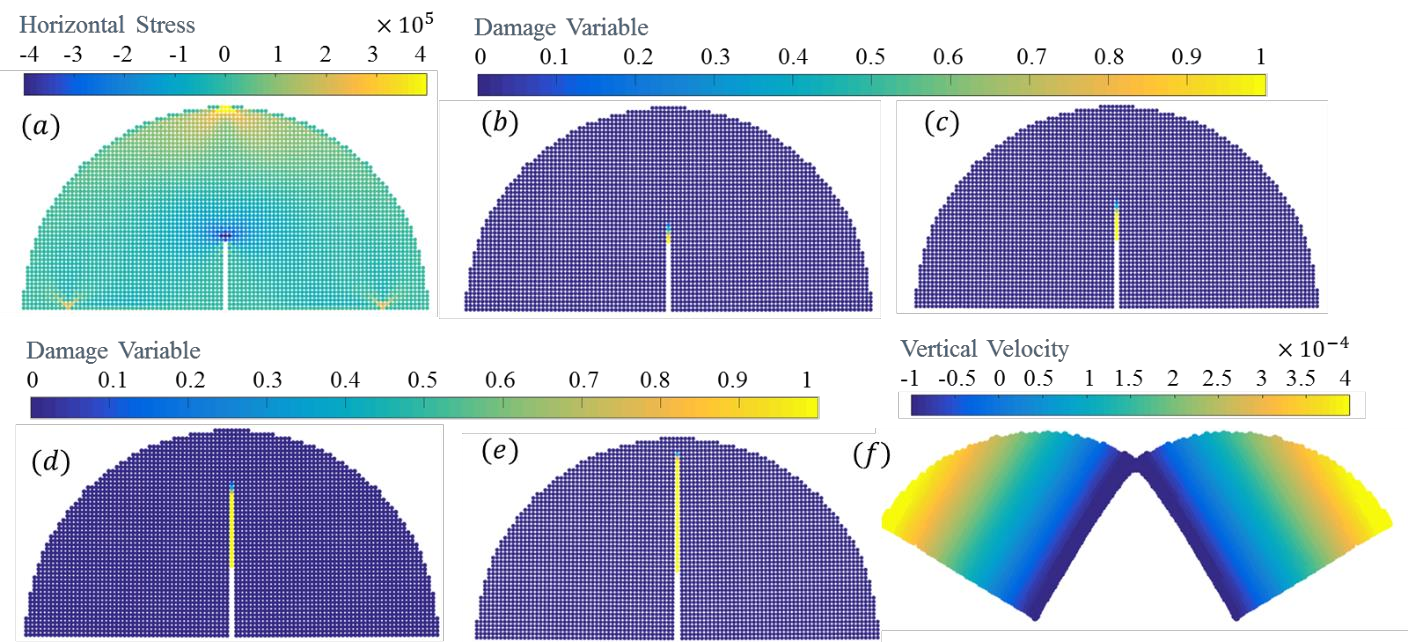
\includegraphics[width=0.95\textwidth]{6-11.png}
\caption{SPH simulation of Johnstone fracture in semi-circular bending test: (a) Horizontal stress profile before fracture; (b-e) Fracture initiation, propagation and final fracture pattern; (f) Profile of vertical velocity at the failure pattern.}\label{fig:6}
\end{figure}

\end{abstract}


%%THE END OF ABSTRACT

\addbib

\end{document}
